\section{Representación}

Dentro del contexto del UTRP, se pretende determinar un conjunto de rutas a partir de distintos paraderos de buses preestablecidos, los cuales deben presentar un beneficio para los pasajeros y para el operador del bus.\\

Para las paradas se utiliza un grafo no dirigido, cuyos vértices corresponden a las paradas y los arcos a un camino entre las paradas. Un ejemplo de esta representación es la red de Mandl, la cual puede apreciarse en la Figura \ref{fig:mandl}.

\begin{figure}[!htb]
\begin{center}
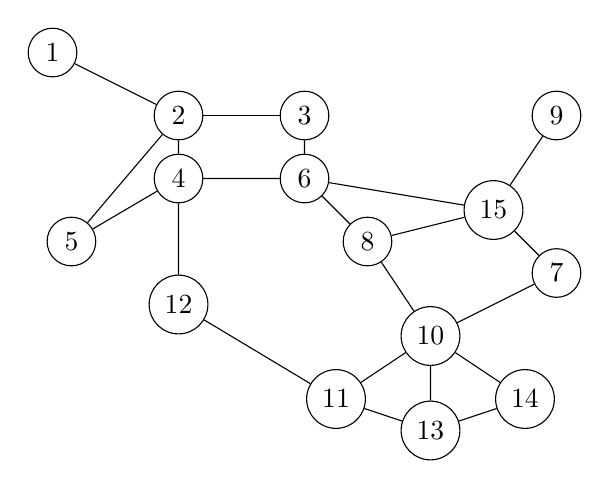
\begin{tikzpicture}[scale=0.8]
\node[draw,circle](1) at (0,0) { 1};
\node[draw,circle](2) at (2,-1) { 2};
\node[draw,circle](3) at (4,-1) { 3};
\node[draw,circle](4) at (2,-2) { 4};
\node[draw,circle](5) at (0.3,-3) { 5};
\node[draw,circle](6) at (4,-2) { 6};
\node[draw,circle](7) at (8,-3.5) { 7};
\node[draw,circle](8) at (5,-3) { 8};
\node[draw,circle](9) at (8,-1) { 9};
\node[draw,circle](10) at (6,-4.5) {10};
\node[draw,circle](11) at (4.5,-5.5) {11};
\node[draw,circle](12) at (2,-4) {12};
\node[draw,circle](13) at (6,-6) {13};
\node[draw,circle](14) at (7.5,-5.5) {14};
\node[draw,circle](15) at (7,-2.5) {15};

\draw (1) -- (2);
\draw (2) -- (3);
\draw (2) -- (4);
\draw (2) -- (5);
\draw (3) -- (6);
\draw (4) -- (5);
\draw (4) -- (6);
\draw (4) -- (12);
\draw (6) -- (8);
\draw (6) -- (15);
\draw (7) -- (15);
\draw (7) -- (10);
\draw (8) -- (10);
\draw (8) -- (15);
\draw (9) -- (15);
\draw (10) -- (11);
\draw (10) -- (13);
\draw (10) -- (14);
\draw (11) -- (12);
\draw (11) -- (13);
\draw (13) -- (14);
\end{tikzpicture}
\caption{Red de Mandl}
\label{fig:mandl}
\end{center}
\end{figure}

La representación escogida para manejar el UTRP es mediante un arreglo bi-dimensional que representa un conjunto de rutas. Cada fila será una ruta, la cual contiene un identificador asociado al número de ruta y posteriormente identificadores para los paraderos de buses. Estos paraderos se encuentran representados por una matriz de demandas, una matriz de tiempos de viaje y por un sistema de coordenadas (este último para modelar la posición de cada paradero).

En la Figura \ref{fig:repr1} se muestra un ejemplo de una representación de rutas el cual se pudo obtener a partir de la literatura existente sobre el UTRP \cite{metaheuristic2010}.

\begin{figure}[!htb]
\begin{center}
\begin{tabular}{|p{0.8cm}|p{0.8cm}|p{0.8cm}|p{0.8cm}|p{0.8cm}|}
\hline
R1 & 0 & 1 & 4 & 7\\
\hline
R2 & 0 & 3 & 6 & $*$\\
\hline
R3 & 1 & 2 & 5 & $*$\\
\hline
\end{tabular}
\caption{Representación para las rutas.}
\label{fig:repr1}
\end{center}
\end{figure}

Las matrices de tiempos de viaje y de demandas se representan mediante arreglos bidimensionales, donde la fila $i$ y columna $j$ aporta información entre el paradero $i$ y el paradero $j$.\\

Las soluciones para el algoritmo inmune artificial propuesto están dadas por un conjunto de rutas que siguen la estructura de la Figura \ref{fig:repr1}.
